\documentclass{article}
\usepackage{graphicx} % Required for inserting images
\usepackage{minted}

\title{Optimisation Algorithms}
\author{Alex Zhou}
\date{May 2019}

\begin{document}

\maketitle

\section{Introduction}

In applied mathematics, statistics and machine learning, it is common to derive estimators and make decisions by minimising some objective function f. Generally, the solution does not have a closed form. One way to approach this is to apply an iterative optimisation algorithm or numerical method to approximate a minimiser. However, problems can have complicated objective functions which admit multiple local minima. It is common practice to run the optimisation algorithm
multiple times from different initial conditions, to eventually find the true global minimiser or perhaps a satisfactory one. It is thus of interest to understand the sensitivity of optimisation algorithms to their initialisation, and to understand which features of the objective function inform the outcomes of these algorithms.

\section{Gradient Descent}

Let \(f: \mathbf{D} \to \mathbf{R}\) be a differentiable objective function with domain \(\mathbf{D} \subset \mathbf{R}^d\), \(d \geq 1\). Set an initial point \(x_0 \in \mathbf{D}\) and a step-size \(h > 0\). The iterates of the gradient descent algorithm are defined recursively as
\[ x_t = x_{t-1} - h\nabla f(x_{t-1}), \quad t \in \mathbf{N}. \]
We desire convergence as \(t \to \infty\), that is \(x_t\) converge to a minimiser \(x_*\) of \(f\) for sufficiently small \(h\).

Let us focus on the double-well function \(f_\theta\) defined for \(\theta \in (0, \pi)\) by
\[ f_\theta: [-1, 1] \to \mathbf{R}, \quad x \mapsto \left(x^2 - \frac{3}{4}\right)^2 - x\cos\theta. \]
Taking the derivative,
\[ f_\theta'(x) = 2\left(x^2 - \frac{3}{4}\right)(2x) - \cos\theta = 4x^3 - 3x - \cos\theta. \]
We recall the triple cosine angle formula
\[ 4\cos^3\phi - 3\cos\phi = \cos3\phi, \]
which shows that the stationary points satisfy
\[ x = \cos\left(\frac{\theta + 2\pi n}{3}\right), \quad n \in \mathbf{Z}. \]
We require \(x \in [-1, 1]\) and it suffices to take \(n = 0,1,2\) by periodicity of the cosine function. Now, computing the second derivative,
\[ f_\theta''(x) = 12x^2 - 3 = 12\cos^2\left(\frac{\theta + 2\pi n}{3}\right) - 3, \]
we can analyse the nature of the stationary points. 
\begin{enumerate}
    \item For \(x_0 = \cos\left(\frac{\theta}{3}\right)\), \(0 < \frac{\theta}{3} < \frac{\pi}{3}\), we have \(\frac{1}{4} < \cos^2\left(\frac{\theta}{3}\right) < 1\), which means \(f_\theta''(x_0) > 0\). Hence \(x_0\) is a local minimum.
    \item For \(x_1 = \cos\left(\frac{\theta + 2\pi}{3}\right)\), \(\frac{2\pi}{3} < \frac{\theta+2\pi}{3} < \pi\), we have \(\frac{1}{4} < \cos^2\left(\frac{\theta+2\pi}{3}\right) < 1\), which means \(f_\theta''(x_1) < 0\). Hence \(x_1\) is a local maximum.
    \item For \(x_2 = \cos\left(\frac{\theta + 4\pi}{3}\right)\), \(\frac{4\pi}{3} < \frac{\theta+4\pi}{3} < \frac{5\pi}{3}\), we have \(0 < \cos^2\left(\frac{\theta+4\pi}{3}\right) < \frac{1}{4}\), which means \(f_\theta''(x_1) < 0\). Hence \(x_1\) is a local maximum.
\end{enumerate}
Note that there are no saddle point for any \(\theta \in (0, \pi)\). We shall use these exact properties and the analytic form of solutions to analyse the performance of the iterative gradient descent algorithm. 

Take \(\theta = \frac{\pi}{6}\) and \(h = 0.01\), let us run the algorithm for \(1000\) steps for each initial point \(x_0 \in \{\frac{k}{50} : k = -50, -49, \dots, 49, 50\}\). The following is a simple implementation in Python:

\begin{minted}[autogobble, linenos]{python}
    def gradient_descent(grad, num_of_steps, step_size, x_initial):
        x_current = x_initial.copy()
        for step in range(num_of_steps):
            x_current -= step_size * grad(x_current)
        return x_current
\end{minted}

We notice that the algorithm converges to the minimum at \(x_1 \approx -0.6428\) for \(x_0 \leq -0.36\) and converges to the minimum at \(x_0 \approx 0.9848\) for \(x \geq -0.36\). We see that when the initial point is to the left of the maximum \(x_2 \approx -0.3420\), then the iteration converges to \(x_1\), whereas if the initial point is to the right of the maximum, then the iteration converges to \(x_0\). Hence, \(x_2\) acts as a separator for the basins of attraction for the two minima.

\section{Monte Carlo Method}

Let \(X\) be a random variable and \(g\) be a function. Consider estimating the quantity
\[ \nu = \mathbf{E}[g(X)]. \]
The Monte Carlo (MC) method involves drawing \(N\) independent random samples \((X^i)_{i=1}^N\) which are identically distributed like \(X\). This now forms the sample mean estimator
\[ \hat\nu_N = \frac{1}{N}\sum_{i=1}^N g(X^i). \]
First, note that this estimator is an unbiased estimator for \(\nu\) as \(\mathbf{E}[g(X^i)] = \mathbf{E}[g(X)] = \nu\), and linearity of expectation yields
\[ \mathbf{E}[\hat\nu_N] = \mathbf{E}\left[\frac{1}{N}\sum_{i=1}^N g(X^i)\right] = \frac{1}{N}\sum_{i=1}^N\mathbf{E}[ g(X^i)] = \frac{1}{N}\sum_{i=1}^N \nu = \nu. \]
Assuming \(\mathbf{Var}(g(X) < \infty\), we compute the variance
\begin{eqnarray*}
    \mathbf{Var}(\hat\nu_N) & = & \mathbf{Var}\left(\frac{1}{N}\sum_{i=1}^N g(X^i)\right) \\
                            & = & \frac{1}{N^2}\mathbf{Var}\left(\sum_{i=1}^N g(X^i)\right) \\
                            & = &  \frac{1}{N^2}\sum_{i=1}^N\mathbf{Var}( g(X^i)) \quad \mbox{(independence)} \\
                            & = &  \frac{1}{N^2}\sum_{i=1}^N\mathbf{Var}( g(X)) \\
                            & = &  \frac{1}{N}\mathbf{Var}( g(X)). \\
\end{eqnarray*}

Returning to our previous function, fix \(\theta \in (0, \pi)\), \(f = f_\theta\) and let \(\{X^h_t\}_{t=0}^\infty\) be the sequence of random variables obtained by sampling an initial point \(X_0^h \sim \mathrm{Unif}[-1, 1]\) and iterating 
\[ X^h_t = X^h_{t-1} - h\nabla f(X^h_{t-1}). \]
For some \(T, h > 0\) such that \(T / h \in \mathbf{N}\), we are interested in examining the behaviour of
\[ \mu^h = \mathbf{E}[X^h_{T/h}] \quad \mbox{and} \quad \mu = \lim_{h \to 0} \mu^h, \]
in other words, the outcome of running gradient descent from a randomised initial point, decreasing step-sizes and increasing iterations. 

Fix \(T = 10\) and \(\theta = \frac{\pi}{4}\). Let us take step-sizes \(h \in \{0.1 \cdot 2^{-k} : k = 0, 1, \dots 10\}\) and estimate \(\mu^h\) using the Monte-Carlo estimator \(\hat{\mu}^h_N\) with \(N = 2^{20-k}\) samples so that the same computational power is used for each \(k\). Indeed, the number of steps per run is \(T / h = 10 / (0.1 \cdot 2^{-k}) = 100 \cdot 2^k\), whilst the number of samples is \(2^{20-k}\), so the total computational effort is the product \(100 \cdot 2^{20}\).

From the previous section, we have the exact formulae of the stationary points for \(\theta = \frac{\pi}{4}\), which turn out to be approximately \(x_0 = 0.9659\), \(x_1 = -0.7071\) and \(x_2 = -0.2588\). As \(k \to \infty\), then the step-size \(h \to 0\) and the number of steps \(n = T / h \to \infty\). Each gradient descent trajectory \(X^h_t\) starting from \(X^h_0\) will converge to one of the local minima, where \(x_2\) acts as the boundary of the basins of attraction. Since \(X^h_0 \sim \mathrm{Unif}[-1, 1]\), the probability of converging to \(x_1\) is 
\[ p_1 = \Pr(X^h_0 < x_2) = \frac{x_2 - (-1)}{1 - (-1)} \approx 0.3706, \]
and the probability of converging to \(x_0\) is 
\[ p_0 = \Pr(X^h_0 > x_2) = \frac{1 - x_2}{2} \approx 0.6294. \]
In the limit, the random variable \(X^h_{T/h}\) takes values \(x_0\) with probability \(p_0\) and \(x_1\) with probability \(p_1\), so
\[ \mu = \lim_{h \to 0} \mu^h = p_0x_0 + p_1x_1 \approx 0.3459. \]
For small \(k\), the step-size \(h\) is large so \(n\) is small which means the gradient descent is not ran very deeply; however, the number of samples \(N\) is large. This means that the approximation \(\hat\mu^{h}_N\) will not be accurate but will be precise. Conversely, for large \(k\), the gradient descent is run for higher iterates, but there are fewer samples, leading to a more accurate but less precise approximation.

Now, considering the variance, as \(h \to 0\) and \(n \to \infty\), note that for \(Y = \lim_{h \to 0} X^h_n\),
\[ \mathbf{E}[Y^2] = p_0x_0^2 + p_1x_1^2, \]
so
\[ \mathbf{Var}(Y) = \mathbf{E}[Y^2] - (\mathbf{E}[Y])^2 = p_0x_0^2 + p_1x_1^2 - (p_0x_0 + p_1x_1)^2 \approx 0.6529. \]
For small \(k\), the variance may be larger due to the gradient descent trajectories not having fully converged. For large \(k\), the variance should stabilise as the \(X^h_n\) start to cluster around the minima, but the estimates for the variance will be noisier due to a lower sample size. The 'between-cluster' variance of the trajectories at two distinct minima forms the dominant part of the variance, but as we increase \(n\), the 'within-variance' of the two clusters becomes tighter.

\begin{minted}[autogobble, linenos]{python}
    def monte_carlo(grad, k, N_func, T, h_base):
        h = h_base / 2**k
        n = int(T / h)
        N = N_func(k)
    
        X_initial = np.random.uniform(-1.0, 1.0, size = N)
        X_final = gradient_descent(grad, n, h, X_initial)
        mu = np.mean(X_final)
        var = np.var(X_final) / N
        return n, N, mu, var
\end{minted}

The table of \(n\), \(N\), mean and variance below seems to suggest the variance is quite stable for both small and large \(k\). This is an artifact of 'trading' the depth of gradient descent for the amount of samples. The tightening of the two clusters is balanced by the the decreasing sample size and vice versa.

\begin{verbatim}[Output]
    n       N           mean                  variance
    100     1048576     0.3470555281684186    0.6523897426576318
    200     524288      0.3443941870869204    0.6535411204278064
    400     262144      0.3463183941281371    0.652710067848017
    800     131072      0.3465545323053242    0.6526075711566739
    1600    65536       0.34795859714624344   0.6519958284113568
    3200    32768       0.3528855883158226    0.6498179744468777
    6400    16384       0.35405989709123875   0.6492917356365032
    12800   8192        0.350996482892206     0.6506587454256023
    25600   4096        0.3601867254869862    0.64650140902388
    51200   2048        0.3450738821088053    0.6532484104354926
    102400  1024        0.35487680754327355   0.6489240298170508
\end{verbatim}

Furthermore, dividing \(\mathbf{Var}(X_n^h)\) by \(N\) yields the variance of \(\hat\mu^h_N\). We can see that as we decrease the step-size \(h\) or equivalently increase the depth of gradient descent \(n\), then the sample size \(N\) decreases, leading to increased variance of the estimator \(\hat\mu^h_N\).

\section{Bias-Variance Tradeoff}

Since \(h\) is not exactly zero, the estimator for the mean incurs some positive finite bias. This means that the Monte-Carlo estimator \(\hat\mu^h_N\) will converge to \(\mu^h \neq \mu\). As such, the variance of the estimator may not fully reflect the accuracy of the approximation. Instead, we use the mean squared error (MSE) which is defined for an estimator \(T\) for a statistic \(\tau\) by
\[ \mathbf{MSE}(T; \tau) = \mathbf{E}[(T - \tau)^2]. \]

There is a well-known decomposition of MSE into the bias and variance
\begin{eqnarray*}
    \mathbf{MSE}(T; \tau) & = & \mathbf{E}[(T - \tau)^2] = \mathbf{E}[(T - \mathbf{E}[T] + \mathbf{E}[T] - \tau)^2] \\
                          & = & \mathbf{E}[(T - \mathbf{E}[T])^2 + 2(T - \mathbf{E}[T])(\mathbf{E}[T] - \tau)  + (\mathbf{E}[T] - \tau)^2] \\
                          & = & \mathbf{E}[(T - \mathbf{E}[T]^2] + 2\mathbf{E}[(T - \mathbf{E}[T])(\mathbf{E}[T] - \tau)]  + \mathbf{E}[(\mathbf{E}[T] - \tau)^2] \\
                          & = & \mathbf{E}[(T - \mathbf{E}[T]^2] + 2(\mathbf{E}[T] - \mathbf{E}[T])(\mathbf{E}[T] - \tau)  + (\mathbf{E}[T] - \tau)^2 \\
                          & = & \mathbf{Var}(T) + \mathbf{Bias}(T; \tau)^2 \\
\end{eqnarray*}
where \(\mathbf{Var}(T) = \mathbf{E}[(T - \mathbf{E}[T]^2]\) and \(\mathbf{Bias}(T; \tau) = (\mathbf{E}[T] - \tau) \).

We present the following facts without proof: for \(h\) sufficiently small, there are constants \(A_1, A_2, A_3 \in (0, \infty)\) such that:
\begin{enumerate}
    \item The bias of the approximation \(\mu^h\) is bounded as \(|\mu^h - \mu| \leq A_1h\).
    \item The variance of \(X^h_{T/h}\) is bounded as \(\mathbf{Var}(X^h_{T/h}) \leq A_2\).
    \item For \(t \in \mathbf{N}\), the cost of generating a sample of \(X^h_t\) satisfies \(\mathbf{Cost}(X^h_t) = A_3t\).
\end{enumerate}

Suppose that we now estimate \(\mu\) by fixing \(h > 0\) and \(N \in \mathbf{N}\) which now does not depend on \(h\), and generate \(N\) independently and identically distributed samples \((Y_i)_{i=1}^N\), distributed as \(X^h_{T/h}\) and forming the estimator
\[ \hat\mu^h_N = \frac{1}{N}\sum_{i=1}^N Y^i. \]
We use the bias-variance decomposition,
\[ \mathbf{MSE}(\hat\mu^h_N; \mu) = \mathbf{Var}[\hat\mu^h_N] + \mathbf{Bias}(\hat\mu^h_N; \mu)^2, \]
to bound the MSE of the estimator from the true mean \(\mu\).

Since \(Y_i\) are identically distributed as \(X^h_{T/h}\), we have \(\mathbf{E}[Y^i] = \mu^h\), so
\[ \mathbf{E}[\hat\mu^h_N] = \mathbf{E}\left[\frac{1}{N}\sum_{i=1}^N Y^i\right] = \frac{1}{N}\sum_{i=1}^N\mathbf{E}[Y^i] = \frac{1}{N}N\mu^h = \mu^h, \]
hence \(\mathbf{Bias}(\hat\mu^h_{N}, \mu) = \mathbf{E}[\hat\mu^h_N] - \mu =  \mu^h - \mu\) which yields the bound
\[ \mathbf{Bias}(\hat\mu^h_N, \mu)^2 = |\mu^h - \mu|^2 \leq (A_1h)^2. \]
Similarly, by independence now as well, \(\mathbf{Var}(Y^i) = \mathbf{Var}(X^h_{T/h})\), so
\[ \mathbf{Var}(\hat\mu^h_N) = \mathbf{Var}\left(\frac{1}{N}\sum_{i=1}^N Y^i\right) = \frac{1}{N^2}\sum_{i=1}^N\mathbf{Var}(Y^i) = \frac{1}{N}\mathbf{Var}(X^h_{T/h}), \]
hence 
\[ \mathbf{Var}(\hat\mu^h_{N}) = \frac{1}{N}\mathbf{Var}(X^h_{T/h}) \leq \frac{A_2}{N}. \]
Altogether, we have
\[ \mathbf{MSE}(\hat\mu^h_N; \mu) \leq A_1^2h^2 + \frac{A_2}{N}. \]
This also confirms our analysis that decreasing \(h\) will decrease the bias, whilst increasing \(N\) will decrease the variance.

Let \(C\) be the computational budget of generating all \(N\) samples. Since the cost of generating one sample \(Y^i \sim X^h_{T/h}\) is \(A_3T/h\), then the total cost is \(N \cdot A_3T/h = C\), assuming we use all our computational power. From this, we can express \(N\) in terms of \(h\) and \(C\),
\[ N = \frac{Ch}{A_3T}, \]
which we substitute into the MSE upper bound
\[ \mathbf{MSE}(\hat\mu^h_{Ch/A_3T}; \mu) \leq A_1^2h^2 + \frac{A_2A_3T}{C}h^{-1}, \]
where this is a function of \(h\). To find the value of \(h\) which minimises the MSE, let
\[ f(h) = A_1^2h^2 + \frac{A_2A_3T}{Ch} \]
and differentiate with respect to \(h\) to obtain
\[ f'(h) = 2A_1^2h - \frac{A_2A_3T}{C}h^{-2}. \]
Setting \(f'(h) = 0\), we have the root
\[ h_* = \sqrt[3]{\frac{A_2A_3T}{2A_1^2C}}. \]
We can verify that \(f''(h) = 2A_1^2 + \frac{2A_2A_3T}{C}h^{-3} \) is positive at \(h_*\), since all constants, variables and terms are positive. Substituting this minimiser back into the upper bound for the MSE, 
\[ \mathbf{MSE}(\hat\mu^{h_*}_{Ch_*/A_3T}; \mu) \leq 3A_1^2\left(\frac{A_2A_3T}{2A_1^2C}\right)^{\frac{2}{3}} = O(C^{-\frac{2}{3}}), \]
that is, the optimal MSE scales with the computational budget \(C\) as \(C^{-2/3}\).

\section{Multi-Level Monte Carlo}

For a given computational budget \(C\), it is possible to construct estimators with less variability than \(\hat\mu^h_N\) which will improve our accuracy. If the initial point \(x_0\) is fixed, then we expect the trajectories of \(X^h_t\) and \(X^{h/2}_{2t}\) to stay reasonably close together, hence \(\mu^h \approx \mu^{h/2}\). We introduce an additional fact to the previous three without proof.
\begin{enumerate}\setcounter{enumi}{3}
    \item If two sequences of gradient descent iterates have the same initial point \(X_0 \sim \mathrm{Unif}[-1, 1]\), then
    \[ \mathbf{Var}(X^h_{T/h} - X^{h/2}_{2T/h}) \leq A_4h^2.  \]
\end{enumerate}
For \(X_0 \sim \mathrm{Unif}[-1, 1]\) and \(l \in 0, \dots, L \in \mathbf{N}\), define \(h_l = 0.1 \cdot 2^{-l}\) and let \(X^{h_l}_{T/h_l}\) be the \(T/h_l\)-th gradient descent iteration for \(f_\theta\) with initial point \(X_0^{h_l} = X_0\) and with step-size \(h_l\). Define the random variables
\[ Y_0 = X^{h_0}_{T/h_0}, \quad Y_l = X^{h_l}_{T/h_l} - X^{h_{l-1}}_{T/h_{l-1}}, \quad l = 1, \dots, L. \]
We can now write
\[ \sum_{l = 0}^L \mathbf{E}[Y_l]. \]
We claim that this sum is absolutely convergent. Since \(Y_0 = X^{h_0}_{T/h_0}\) we have \(\mathbf{E}[Y_0] = \mu^{h_0}\), and similarly, for \(l = 1, \dots, L\), 
\[  Y_l = X^{h_l}_{T/h_l} - X^{h_{l-1}}_{T/h_{l-1}}  \Rightarrow \mathbf{E}[Y_l] = \mu^{h_l} - \mu^{h_{l-1}}. \]
Consider the terms \(|\mathbf{E}[Y_l]|\). For \(l=0\), \(|\mathbf{E}[Y_0]| = |\mu^{h_0}|\) and 
\[ |\mu^{h_0} - \mu| \leq A_1 h_0. \]
Since \(\mu\) is the limit of \(\mu^h\) and \(h_0\) is fixed, if \(\mu\) is finite then \(|\mu^{h_0}|\) is finite. More generally, for \(l \geq 1\), we have \(|\mathbf{E}[Y_l]| = |\mu^{h_l} - \mu^{h_{l-1}}|\). Using the triangle inequality, 
\[ |\mu^{h_l} - \mu^{h_{l-1}}| = |\mu^{h_l} - \mu - \mu^{h_{l-1}} - \mu| \leq |\mu^{h_l} - \mu| + |\mu^{h_{l-1}} - \mu|, \]
hence \(|\mathbf{E}[Y_l]| \leq A_1 h_l + A_1 h_{l-1}\). Given \(h_l = 0.1 \cdot 2^{-l}\), we have 
\[ h_{l-1} = 0.1 \cdot 2^{-(l-1)} = 0.1 \cdot 2 \cdot 2^{-l} = 2h_l, \]
therefore,
\[ |\mathbf{E}[Y_l]| \leq A_1 h_l + A_1 (2h_l) = 3A_1 h_l. \]

Now,
\begin{eqnarray*} 
    \sum_{l=0}^\infty |\mathbf{E}[Y_l]| & = & |\mathbf{E}[Y_0]| + \sum_{l=1}^\infty |\mathbf{E}[Y_l]| \\ 
                                        & \leq & |\mu^{h_0}| + \sum_{l=1}^\infty 3A_1 h_l \\
                                        & \leq & |\mu^{h_0}| + \sum_{l=1}^\infty 3A_1 (0.1 \times 2^{-l}) \\
                                        & = & |\mu^{h_0}| + 0.3 A_1 \sum_{l=1}^\infty \left(\frac{1}{2}\right)^l. 
\end{eqnarray*}
The geometric series converges as \(\frac{1}{2} < 1\), and 
\[ \sum_{l=1}^\infty \left(\frac{1}{2}\right)^l = \frac{1/2}{1 - 1/2} = 1. \]
So, \(\sum_{l=0}^\infty |\mathbf{E}[Y_l]| \leq |\mu^{h_0}| + 0.3 A_1 < \infty\). Thus, the series \(\sum_{l \ge 0} \mathbf{E}[Y_l]\) converges absolutely, as required.

To find an upper bound for the truncation error incurred by approximating \(\mu \approx \sum_{l=0}^L \mathbf{E}[Y_l]\), the sum \(\sum_{l=0}^L \mathbf{E}[Y_l]\) is a telescoping sum for the expectations,
\begin{eqnarray*}
    \sum_{l=0}^L \mathbf{E}[Y_l] & = & \mathbf{E}[Y_0] + \sum_{l=1}^L (\mathbf{E}[X^{h_l}_{T/h_l}] - \mathbf{E}[X^{h_{l-1}}_{T/h_{l-1}}]) \\
    & = & \mu^{h_0} + (\mu^{h_1} - \mu^{h_0}) + (\mu^{h_2} - \mu^{h_1}) + \dots + (\mu^{h_L} - \mu^{h_{L-1}}) = \mu^{h_L}. 
\end{eqnarray*}
Thus, the truncation error is bounded from above by \(|\mu - \mu^{h_L}| \leq A_1h_l = A_1 (0.1 \cdot 2^{-L})\).

With this in mind, we aim to approximate \(\mu\) by taking some truncation level \(L\), a sequence of level sizes \((N_l)_{l=1}^L\) and forming the multi-level Monte Carlo (MLMC) estimator 
\[ \hat\mu_{N_{1:L}} = \sum_{l=0}^L \left(\frac{1}{N_l} \sum_{i=1}^{N_l} Y_l^i\right), \]
where for each \(i\), \((Y_l^i)_{i=1}^{N_l}\) are independent, identically distributed samples of \(Y^i\). In order words, for each \((i,l)\), we dependently draw an initial point \(X_0^{(i,l)} \sim \mathrm{Unif}[-1, 1]\) and define \(Y^i_l\) using \(X_0^{(i,l)}\) instead of \(X_0\). Hence \((Y_l^i)_{i,l}\) are mutually independent.

Let \(\theta \in \{ k\pi / 2^7 : k = 1, \dots, 2^6 \}\). Let us fix \(L = 10\), \(T = 10\) with level sizes \(N_l = 5\) and \(N_l = 2^{L-l}\). For the latter, notice that we put the most weight on the low-cost \(Y_0\) iteration, and less weight on the higher-cot iterations. We use the following Python code:

\begin{minted}[autogobble, linenos]{python}
    def multi_level_monte_carlo(grad, L, N_func_l, T, h_base):
        mu_estimate = 0.0
    
        h_0 = h_base
        n_0 = int(T / h_0)
        N_0 = N_func_l(0, L)
        X_initial_0 = np.random.uniform(-1.0, 1.0, size = N_0)
        Y_0 = gradient_descent(grad, n_0, h_0, X_initial_0)
        mu_estimate += np.mean(Y_0)
    
        for l in range(1, L + 1):
            h_l = h_base / 2**l
            n_l = int(T / h_l)
            N_l = N_func_l(l, L)
            X_initial_l = np.random.uniform(-1.0, 1.0, size = N_l)
            X_fine_l = gradient_descent(grad, n_l, h_l, X_initial_l)
            X_coarse_l = gradient_descent(grad, n_l // 2, 2 * h_l , X_initial_l)
            Y_l = X_fine_l - X_coarse_l
            mu_estimate += np.mean(Y_l)
        return mu_estimate
\end{minted}

The variance of \(\hat{\mu}_{N_{1:L}} = \sum_{l=0}^L \left(\frac{1}{N_l} \sum_{i=1}^{N_l} Y_l^i\right) = \sum_{l=0}^L \hat Y_l\) is given by
\[ \mathbf{Var}(\hat{\mu}_{N_{1:L}}) = \mathbf{Var}\left(\sum_{l=0}^L \hat Y_l \right) = \sum_{l=0}^L \frac{1}{N_l}\mathbf{Var}(Y_l). \]
We expect the variance of \(Y_l\) to decay quadratically as \(l\) increases. The dominant term is therefore expected to be \(Y_0\). For \(N_l = 5\), we expect the variance to be very high since the variance is dominated by \(\mathbf{Var}(Y_0)/5\). For \(N_l = 2^{L-l}\), this choice aims to balance the larger variance at \(Y_0\) with a larger number of samples, resulting in a lower variance. This is demonstrated through the plots below, where the former has high oscillations but the second looks much smoother.

\begin{figure}
    \centering
    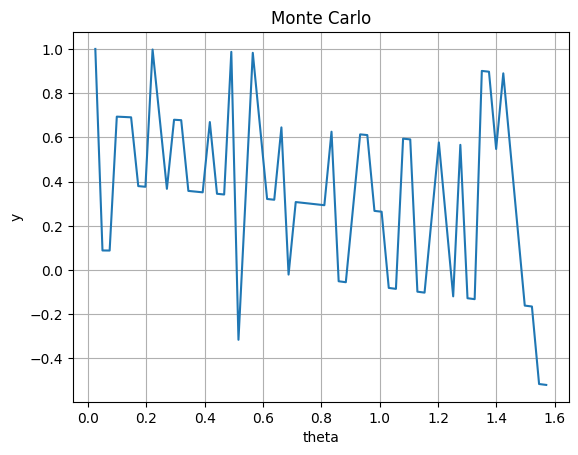
\includegraphics[width=0.45\linewidth]{images/N1var.png}
    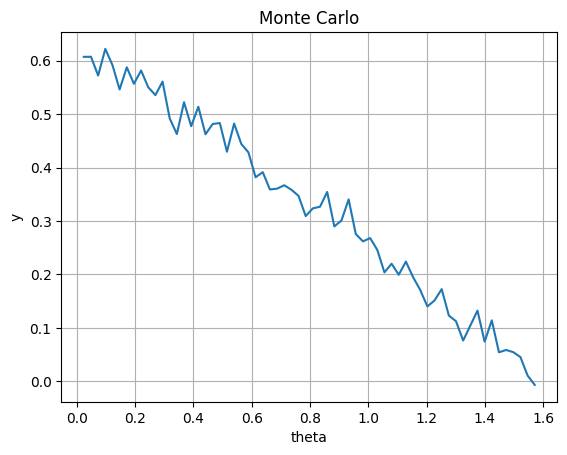
\includegraphics[width=0.45\linewidth]{images/N2var.png}
    \caption{Plot of \(y = \hat\mu_{N_{1:L}}\) over \(\theta\) for \(N_l = 5\) and \(N_l = 2^{L-l}.\)}
\end{figure}

Next, we derive an upper bound for the mean square error of the MLMC estimator. We use the bias-variance decomposition
\[ \mathbf{MSE}(\hat\mu_{N_{1:L}}; \mu) = \mathbf{Bias}(\hat\mu_{N_{1:L}}; \mu)^2 + \mathbf{Var}(\hat\mu_{N_{1:L}}). \]
For the bias term, recall \(\hat Y_l := \frac{1}{N_l}\sum_{i=1}^{N_l} Y_l^{(i,l)}\), so
\begin{eqnarray*} 
    \mathbf{Bias}(\hat\mu_{N_{1:L}}; \mu) & = & \mathbf{E}[\hat\mu_{N_{1:L}}] - \mu \\
                                          & = & \sum_{l=1}^L\mathbf{E}[\hat Y_l] - \mu \\
                                          & = & \sum_{l=1}^L\mathbf{E}[Y_l] - \mu \\
                                          & = & \mu^{h_L} - \mu,
\end{eqnarray*}
which yields the estimate 
\[\mathbf{Bias}(\hat\mu_{N_{1:L}}; \mu) \leq A_1h_L. \] 
For the variance term, by independence, 
\[ \mathbf{Var}(\hat\mu_{N_{1:L}}; \mu) = \mathbf{Var}\left(\sum_{l=0}^L \hat Y_l\right) = \sum_{l=0}^L \mathbf{Var}(\hat Y_l) = \sum_{l=0}^L\frac{1}{N_l}\mathbf{Var}(Y_l). \]
For \(l = 0\), \(\mathbf{Var}(Y_0) \leq A_2\) and for \(l \geq 1\) since \(2h_l = h_{l-1}\) and \(X^{h/2}_{2T/h}\) and \(X^h_{T/h}\) start from the same \(X_0\), we have the bound \(\mathbf{Var}(Y_l) \leq A_4h_{l-1}^2\). Therefore
\[ \mathbf{Var}(\hat\mu_{N_{1:L}}; \mu) \leq \frac{A_2}{N_0} + \sum_{l=1}^L \frac{A_4h_{l-1}^2}{N_l}. \]
Altogether, 
\[ \mathbf{MSE}(\hat\mu_{N_{1:L}}; \mu) \leq A_1^2h_L^2 + \frac{A_2}{N_0} + \sum_{l=1}^L\frac{A_4h_{l-1}^2}{N_l}. \]
Using this upper bound, we will now try to choose \(L\) and \((N_l)_{l=0}^L\) such that the MSE of the corresponding MLMC estimator is minimised, given a fixed computational budget \(C\). We treat all \(N_l\) as continuous variables and set \(L = \infty\) for simplicity. 

We have the following minimisation problem:
\[ \mbox{Minimise} \quad F((N_l)_{l=0}^\infty) = \sum_{l=0}^\infty \frac{V_l}{N_l} \quad \mbox{subject to} \quad \sum_{l=0}^\infty N_lC_l = C, \]
where \(C_l\) is the cost per sample at level \(l\), \(V_0 = A_2\) and \(V_l = A_4h_{l-1}^2\) for \(l \geq 1\). Note that
\[ C_0 = \mathbf{Cost}(Y_0) = \mathbf{Cost}(X^{h_0}_{T/h_0}) = \frac{A_3T}{h_0},  \]
and for \(l \geq 1\),
\[ C_l = \mathbf{Cost}(Y_l) = \mathbf{Cost}(X^{h_l}_{T/h_l}) + \mathbf{Cost}(X^{h_{l-1}}_{T/h_{l-1}}) = \frac{A_3T}{h_l} + \frac{A_3T}{h_{l-1}} = \frac{3A_3T}{2h_l}.  \]
Formulating the problem in terms of Lagrange multipliers,
\[ H((N_l)_{l=0}^\infty, \lambda) = \sum_{l=0}^\infty \frac{V_l}{N_l} + \lambda\left(\sum_{l=0}^\infty N_lC_l - C\right). \]
Differentiating with respect to each \(N_l\) and \(\lambda\),
\[ \frac{\partial H}{\partial N_l} = -\frac{V_l}{N^2_l} + \lambda C_l = 0, \quad \frac{\partial H}{\partial \lambda} = \sum_{l=0}^\infty N_lC_l - C = 0. \]
This implies \(N_l = \sqrt{\frac{V_l}{\lambda C_l}}\) and the Lagrange multiplier is \(\lambda = \frac{1}{C^2}\left(\sum_{l=0}^\infty \sqrt{V_lC_l}\right)^2\). Substituting into the expression for \(N_l\) gives the optimal allocation of \(\tilde{N}_l\),
\[ \tilde{N}_l = \frac{C}{\sum_{k=0}^\infty \sqrt{V_kC_k}} \sqrt{\frac{V_l}{C_l}}. \]

To incorporate the bias term, we now take \(L\) to be finite. Our new optimised upper bound for the MSE after substituting for \(N_l = \lfloor \tilde{N}_l \rfloor\) is now
\[ A_1^2h_L^2 + \frac{1}{C}\left(\sum_{l=0}^L \sqrt{V_lC_l}\right)^2, \]
for which \(L\) can be chosen to minimise the first term coming from squared bias. Note that the sum converges because \(V_k = O(h_k^2)\) and \(C_k = O(1/h_k)\) for large \(k\), hence \(\sqrt{V_kC_k} = O(\sqrt{h_k})\) forms a convergence geometric series by definition of \(h_k\).

To minimise the MSE, the squared bias term and the variance term are typically balanced, \(A_1^2h_L^2 \approx \frac{1}{C} \sum_{l=0}^L \sqrt{V_lC_l}\), i.e. \(h_L = h_0/2^L \approx \frac{1}{A_1\sqrt{C}}\sum_{l=0}^L \sqrt{V_lC_l}\). Taking logarithms yields
\[ L \approx \log_2\left(\frac{A_1h_0}{\sum_{l=0}^L \sqrt{V_lC_l}}\right) + \log_2(\sqrt{C}) = O(\log C). \]
Furthermore, when the terms are balanced the optimal MSE scales with \(C\) as \(O(C^{-1})\). This is noticeably better than the previous MC estimator which scaled with \(C\) as \(O(C^{-\frac{2}{3}})\). In conclusion, the MLMC method achieves a faster rate of convergence for its MSE with respect to the computational budget \(C\).

\section{Application to the Double-Well Loss Function}

We shall now use the estimators defined above to study the behaviour of gradient descent on the double-well function \(f_\theta\) defined earlier. Define \(m_1(\theta) < m_2(\theta)\) as the local minima of \(f_\theta\) in \([-1, 1]\), Suppose that \(h > 0\) and \(T \in \mathbf{N}\) are sufficiently small and large respectively so that
\[ \min{|m_1(\theta) - X^h_T|, \quad |m_2(\theta) - X^h_T|} \approx 0, \]
for any initial point \(x_0 \in [-1, 1]\). Define
\[ p_1(\theta) = \Pr\left(\lim_{T \to \infty} X^h_T = m_1(\theta)\right), \quad p_2(\theta) = \Pr\left(\lim_{T \to \infty} X^h_T = m_1(\theta)\right). \]
Since each trajectory of gradient descent converges to exactly one of the to minima, i.e. the events are mutually exclusive, then 
\[ p_1(\theta) + p_2(\theta) = 1. \]
The expected value of the limiting position is then
\[ \mu(\theta) = m_1(\theta)p_1(\theta) + m_2(\theta)p_2(\theta). \]
Solving this linear system, we derive expressions of \(p_1\) and \(p_2\) in terms of \(\mu\), \(m_1\) and \(m_2\),
\[ p_1 = \frac{m_2 - \mu}{m_2 - m_1}, \quad p_1 = \frac{\mu - m_1}{m_2 - m_1}.  \]
Recall that \(m_1(\theta) = \cos\frac{\theta + 2\pi}{3}\) and \(m_2 = \cos\frac{\theta}{3}\). We will use the MLMC scheme to compute the estimate \(\hat\mu(\theta)\) for \(\theta \in (\frac{k\pi}{2^7})_{k=1}^{2^6}\). We take \(T = 10\), \(L = 10\) and \(N_l = \lfloor 2^{3(L-l)/2}\rfloor\). This choice of \(N_l\) is justified as the optimal allocation \(\tilde{N}_l\) scales like \(\sqrt{V_l/C_l}\) which in turns scales like
\[ \sqrt{\frac{h_l^2}{h_{l}^{-1}}} = \sqrt{h_l^3} = h^{3/2}, \]
so \(\tilde{N}_l \propto K\cdot2^{-3l/2}, \) for \(l \geq 0\).

\begin{figure}
    \centering
    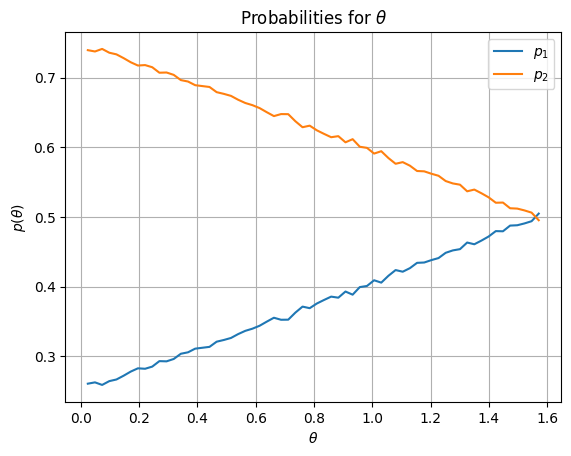
\includegraphics[width=1.0\linewidth]{images/probabilities.png}
    \caption{Estimates of \(p_1(\theta)\) and \(p_2(\theta)\) over \(\theta\).}
\end{figure}

We notice that the sum of the graphs is close to \(1\) as expected. The outcome of the gradient descent algorithm on \(f_\theta\) varies the most when the probability of converging to either minimum is roughly equal, \(p_1(\theta) \approx p_2(\theta) \approx \frac{1}{2}\). Indeed, recall that the variance of the outcome of gradient descent \(Y = \lim_{h\to 0} X_T^h\) is
\[ \mathbf{Var}(Y) = m_1^2p_1 + m_2^2p_2 - (m_1p_1 + m_2p_2)^2=  p_1(1-p_1)(m_1-m_2)^2, \]
which is maximised at \(p_1 = \frac{1}{2}\). The separator of the basins of attraction occur at \(\cos\frac{\theta + 4\pi}{3}\), which is equal to \(0\) when \(\theta = \frac{\pi}{2} \in [0, \pi]\) which is the right-most endpoint of our plot.

\section{Machine Learning in Python}

Python is a popular language used for machine learning owing to its readability and abundance of libraries. Some examples are Scikit-Learn, TensorFlow, PyTorch, Keras and XGBoost.

\end{document}